\documentclass[a4paper, 10pt, french]{article}
% Préambule; packages qui peuvent être utiles
   \RequirePackage[T1]{fontenc}        % Ce package pourrit les pdf...
   \RequirePackage{babel,indentfirst}  % Pour les césures correctes,
                                       % et pour indenter au début de chaque paragraphe
   \RequirePackage[utf8]{inputenc}   % Pour pouvoir utiliser directement les accents
                                     % et autres caractères français
   \RequirePackage{lmodern,tgpagella} % Police de caractères
   \textwidth 17cm \textheight 25cm \oddsidemargin -0.24cm % Définition taille de la page
   \evensidemargin -1.24cm \topskip 0cm \headheight -1.5cm % Définition des marges
   \RequirePackage{latexsym}                  % Symboles
   \RequirePackage{amsmath}                   % Symboles mathématiques
   \RequirePackage{tikz}   % Pour faire des schémas
   \RequirePackage{graphicx} % Pour inclure des images
   \RequirePackage{listings} % pour mettre des listings
% Fin Préambule; package qui peuvent être utiles

\title{Rapport de TP 4MMAOD : Génération de patch optimal}
\author{
MAHIEU LUCAS étudiant$_1$ (SLE\_PHELMA$_1$) 
\\ ANOUFA Guillaume étudiant$_2$ (SLE\_PHELMA$_2$) 
}

\begin{document}

\maketitle

%%%%%%%%%%%%%%%%%%%%%%%%%%%%%%%%%%%%%%%%%%%%%%
\paragraph{\em Préambule}
{\em \begin{itemize} 
   \item Compléter ce patr
\end{itemize}
}

%%%%%%%%%%%%%%%%%%%%%%%%%%%%%%%%%%%%%%%%%%%%%%
\section{Principe de notre  programme (1 point)}
{Nous avons choisi d'implementer un algorithme itératif car cela nous paraissait plus efficace qu'un algorithme récursif qui aurait du faire un très grand nombre d'appel et potentiellement remplir entièrement la pile, pour des fichiers volumineux.
\\ \indent Ainsi nous parcourons une à une toutes les configurations de fichier possible : de $A_0$,$B_0$ à $A_n$,$B_n$, et mémorisons le cout de la configuration à chaque itération.
\\ \indent Pour pouvoir retrouver, à la fin, par quelle configuration nous sommes arrivé à $A_n$,$B_n$, nous mémorisons aussi les indices de la configuration mère ainsi que la chaine de caractère qu'il faudra afficher dans le patch dans le cas ou celui-ci passe par cette configuration.
\\ \indent Pour mémoriser ces informations, nous avons utiliser un tableau de taille (n+1)*(m+1) qui contient des structures appelées 'cellule'. Elles sont définies comme ceci:
{\em \\typedef struct  \{
\\ \indent int cout,
\\ \indent char* cmd,
\\ \indent int pereI,
\\ \indent int pereJ \} cellule;}
\\ \indent Pour mieux comprendre nous avons schématiser ce que notre algorithme fait pour l'exemple du sujet. Voir figure~\ref{étiquette} page~\pageref{étiquette} 

\begin{figure}[!h]
\hspace{2cm}
	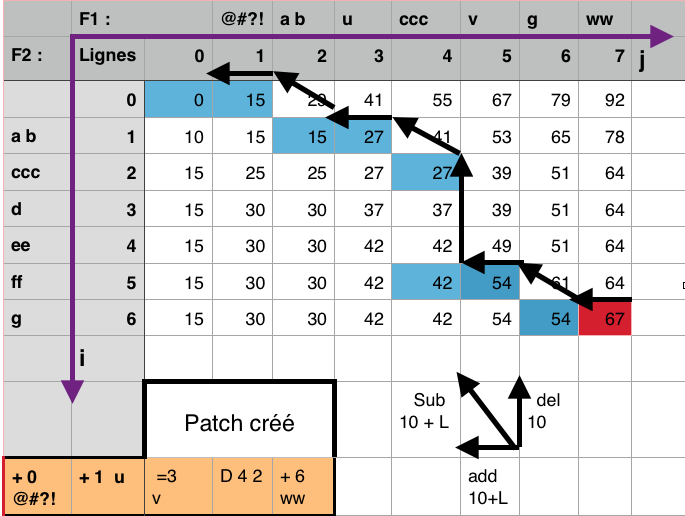
\includegraphics[scale=0.5]{tableau_mem.png}
	\caption{\label{étiquette} Exemple de parcours itératif de notre algorythme pour l'exemple du sujet}
\end{figure}
 \indent Notre algorithme commence dans l'état $A_0$,$B_0$ et calcule colonne par colonne tous les coûts de toutes des configurations. Pour ce faire, à l'étape $A_i$,$B_j$, le coût sera : \\ min \{ ($A_{i-1}$,$B_{j-1}$) + 10+L, ($A_i$,$B_{j-1}$) + 10+L, min\{ ($A_{i-k}$,$B_j$) + 15\} \}
 \\ C'est ce que représente partiellement la figure en bas à droite de la figure~\ref{étiquette} page~\pageref{étiquette} 
 \\ \indent Lorsque l'on arrive dans l'état $A_n$,$B_m$, on va remonter le chemin des pères. Donc en $A_i$,$B_j$ on ira en $A_{péreI}$,$B_{péreJ}$ en {\em 'échangeant'} la valeur des pères pour qu'une fois en $A_0$,$B_0$ on puisse redescendre en $A_n$,$B_m$ par le chemin de coût optimal tout en l'affichant.
 } 

%%%%%%%%%%%%%%%%%%%%%%%%%%%%%%%%%%%%%%%%%%%%%%
\section{Analyse du coût théorique (3 points)}
{\em Donner ici l'analyse du coût théorique de votre programme en fonction des nombres $n_1$ et $n_2$ de lignes 
et $c_1$ et $c_2$ de caractères des deux fichiers en entrée.
 Pour chaque coût, donner la formule qui le caractérise (en justifiant brièvement pourquoi cette formule correspond à votre programme), 
 puis l'ordre du coût en fonction de $n_1, n_2, c_1, c_2$ en notation $\Theta$ de préférence, sinon $O$.}

  \subsection{Nombre  d'opérations en pire cas\,: }
    \paragraph{Justification\,: }
    {\em La justification peut être par exemple de la forme: \\ 
       "Le programme itératif contient les boucles $k_1=...$, $k_2= ...$ etc correspondant à la somme 
      $$T(n_1, n_2, c_1, c_2) = \sum_{k_1=...}^{...} ... \sum ... + \sum_{i=...}^{...} ...$$ 
      somme que nous avons calculée (ou majorée) par la technique de  ... " \\
      ou  encore\,:  \\
      "les appels récursifs du programme permettent de modéliser son coût par le système d'équations aux récurrences 
      $$T(k_1, k_2) = ...  \mbox{~avec~les~conditions~initiales~....~} $$
      Le coût indiqué est obtenu en résolvant ce système par la méthode de  .... "
    } 
  \subsection{Place mémoire requise\,: }
    \paragraph{Justification\,: }
    {
    	Comme la partie 1 l'explique, nous stockons en mémoire (n+1)*(m+1) états.
    }

  \subsection{Nombre de défauts de cache sur le modèle CO\,: }
    \paragraph{Justification\,: }


%%%%%%%%%%%%%%%%%%%%%%%%%%%%%%%%%%%%%%%%%%%%%%
\section{Compte rendu d'expérimentation (2 points)}
  \subsection{Conditions expérimentaless}
     {\em Décrire les conditions permettant la reproductibilité des mesures: on demande la description
      de la machine et la méthode utilisée pour mesurer le temps.
     }

    \subsubsection{Description synthétique de la machine\,:} 
      {\em indiquer ici le  processeur et sa fréquence, la mémoire, le système d'exploitation. 
       Préciser aussi si la machine était monopolisée pour un test, ou notamment si 
       d'autres processus ou utilisateurs étaient en cours d'exécution. 
      } 

    \subsubsection{Méthode utilisée pour les mesures de temps\,: } 
      {\em préciser ici  comment les mesures de temps ont été effectuées (fonction appelée) et l'unité de temps; en particulier, 
       préciser comment les 5 exécutions pour chaque test ont été faites (par exemple si le même test est fait 5 fois de suite, ou si les tests sont alternés entre
       les mesures, ou exécutés en concurrence etc). 
      }

  \subsection{Mesures expérimentales}
    {\em Compléter le tableau suivant par les temps d'exécution mesurés pour chacun des 6 benchmarks imposés
              (temps minimum, maximum et moyen sur 5 exécutions)
    }

    \begin{figure}[h]
      \begin{center}
        \begin{tabular}{|l||r||r|r|r||}
          \hline
          \hline
            & coût         & temps     & temps   & temps \\
            & du patch     & min       & max     & moyen \\
          \hline
          \hline
            benchmark1 &      &     &     &     \\
          \hline
            benchmark2 &      &     &     &     \\
          \hline
            benchmark3 &      &     &     &     \\
          \hline
            benchmark4 &      &     &     &     \\
          \hline
            benchmark5 &      &     &     &     \\
          \hline
            benchmark6 &      &     &     &     \\
          \hline
          \hline
        \end{tabular}
        \caption{Mesures des temps minimum, maximum et moyen de 5 exécutions pour les 6 benchmarks.}
        \label{table-temps}
      \end{center}
    \end{figure}

\subsection{Analyse des résultats expérimentaux}
{\em Donner  une réponse justifiée  à la question\,: 
              les  temps mesurés correspondent ils  à votre analyse théorique (nombre d’opérations et défauts de cache) ?
}

%%%%%%%%%%%%%%%%%%%%%%%%%%%%%%%%%%%%%%%%%%%%%%
\section{Question\,: et  si le coût d'un patch était sa taille en octets ? (1 point)}
{\em Préciser le principe de la résolution choisie (parmi celles vues en cours); donner  les modifications à apporter (soit à vos  équations, soit à votre programme, au choix) 
pour s'adapter à cette nouvelle fonction de coût. 
}

\end{document}
%% Fin mise au format

